\documentclass[1p]{elsarticle_modified}
%\bibliographystyle{elsarticle-num}

%\usepackage[colorlinks]{hyperref}
%\usepackage{abbrmath_seonhwa} %\Abb, \Ascr, \Acal ,\Abf, \Afrak
\usepackage{amsfonts}
\usepackage{amssymb}
\usepackage{amsmath}
\usepackage{amsthm}
\usepackage{scalefnt}
\usepackage{amsbsy}
\usepackage{kotex}
\usepackage{caption}
\usepackage{subfig}
\usepackage{color}
\usepackage{graphicx}
\usepackage{xcolor} %% white, black, red, green, blue, cyan, magenta, yellow
\usepackage{float}
\usepackage{setspace}
\usepackage{hyperref}

\usepackage{tikz}
\usetikzlibrary{arrows}

\usepackage{multirow}
\usepackage{array} % fixed length table
\usepackage{hhline}

%%%%%%%%%%%%%%%%%%%%%
\makeatletter
\renewcommand*\env@matrix[1][\arraystretch]{%
	\edef\arraystretch{#1}%
	\hskip -\arraycolsep
	\let\@ifnextchar\new@ifnextchar
	\array{*\c@MaxMatrixCols c}}
\makeatother %https://tex.stackexchange.com/questions/14071/how-can-i-increase-the-line-spacing-in-a-matrix
%%%%%%%%%%%%%%%

\usepackage[normalem]{ulem}

\newcommand{\msout}[1]{\ifmmode\text{\sout{\ensuremath{#1}}}\else\sout{#1}\fi}
%SOURCE: \msout is \stkout macro in https://tex.stackexchange.com/questions/20609/strikeout-in-math-mode

\newcommand{\cancel}[1]{
	\ifmmode
	{\color{red}\msout{#1}}
	\else
	{\color{red}\sout{#1}}
	\fi
}

\newcommand{\add}[1]{
	{\color{blue}\uwave{#1}}
}

\newcommand{\replace}[2]{
	\ifmmode
	{\color{red}\msout{#1}}{\color{blue}\uwave{#2}}
	\else
	{\color{red}\sout{#1}}{\color{blue}\uwave{#2}}
	\fi
}

\newcommand{\Sol}{\mathcal{S}} %segment
\newcommand{\D}{D} %diagram
\newcommand{\A}{\mathcal{A}} %arc


%%%%%%%%%%%%%%%%%%%%%%%%%%%%%5 test

\def\sl{\operatorname{\textup{SL}}(2,\Cbb)}
\def\psl{\operatorname{\textup{PSL}}(2,\Cbb)}
\def\quan{\mkern 1mu \triangleright \mkern 1mu}

\theoremstyle{definition}
\newtheorem{thm}{Theorem}[section]
\newtheorem{prop}[thm]{Proposition}
\newtheorem{lem}[thm]{Lemma}
\newtheorem{ques}[thm]{Question}
\newtheorem{cor}[thm]{Corollary}
\newtheorem{defn}[thm]{Definition}
\newtheorem{exam}[thm]{Example}
\newtheorem{rmk}[thm]{Remark}
\newtheorem{alg}[thm]{Algorithm}

\newcommand{\I}{\sqrt{-1}}
\begin{document}

%\begin{frontmatter}
%
%\title{Boundary parabolic representations of knots up to 8 crossings}
%
%%% Group authors per affiliation:
%\author{Yunhi Cho} 
%\address{Department of Mathematics, University of Seoul, Seoul, Korea}
%\ead{yhcho@uos.ac.kr}
%
%
%\author{Seonhwa Kim} %\fnref{s_kim}}
%\address{Center for Geometry and Physics, Institute for Basic Science, Pohang, 37673, Korea}
%\ead{ryeona17@ibs.re.kr}
%
%\author{Hyuk Kim}
%\address{Department of Mathematical Sciences, Seoul National University, Seoul 08826, Korea}
%\ead{hyukkim@snu.ac.kr}
%
%\author{Seokbeom Yoon}
%\address{Department of Mathematical Sciences, Seoul National University, Seoul, 08826,  Korea}
%\ead{sbyoon15@snu.ac.kr}
%
%\begin{abstract}
%We find all boundary parabolic representation of knots up to 8 crossings.
%
%\end{abstract}
%\begin{keyword}
%    \MSC[2010] 57M25 
%\end{keyword}
%
%\end{frontmatter}

%\linenumbers
%\tableofcontents
%
\newcommand\colored[1]{\textcolor{white}{\rule[-0.35ex]{0.8em}{1.4ex}}\kern-0.8em\color{red} #1}%
%\newcommand\colored[1]{\textcolor{white}{ #1}\kern-2.17ex	\textcolor{white}{ #1}\kern-1.81ex	\textcolor{white}{ #1}\kern-2.15ex\color{red}#1	}

{\Large $\underline{11n_{148}~(K11n_{148})}$}

\setlength{\tabcolsep}{10pt}
\renewcommand{\arraystretch}{1.6}
\vspace{1cm}\begin{tabular}{m{100pt}>{\centering\arraybackslash}m{274pt}}
\multirow{5}{120pt}{
	\centering
	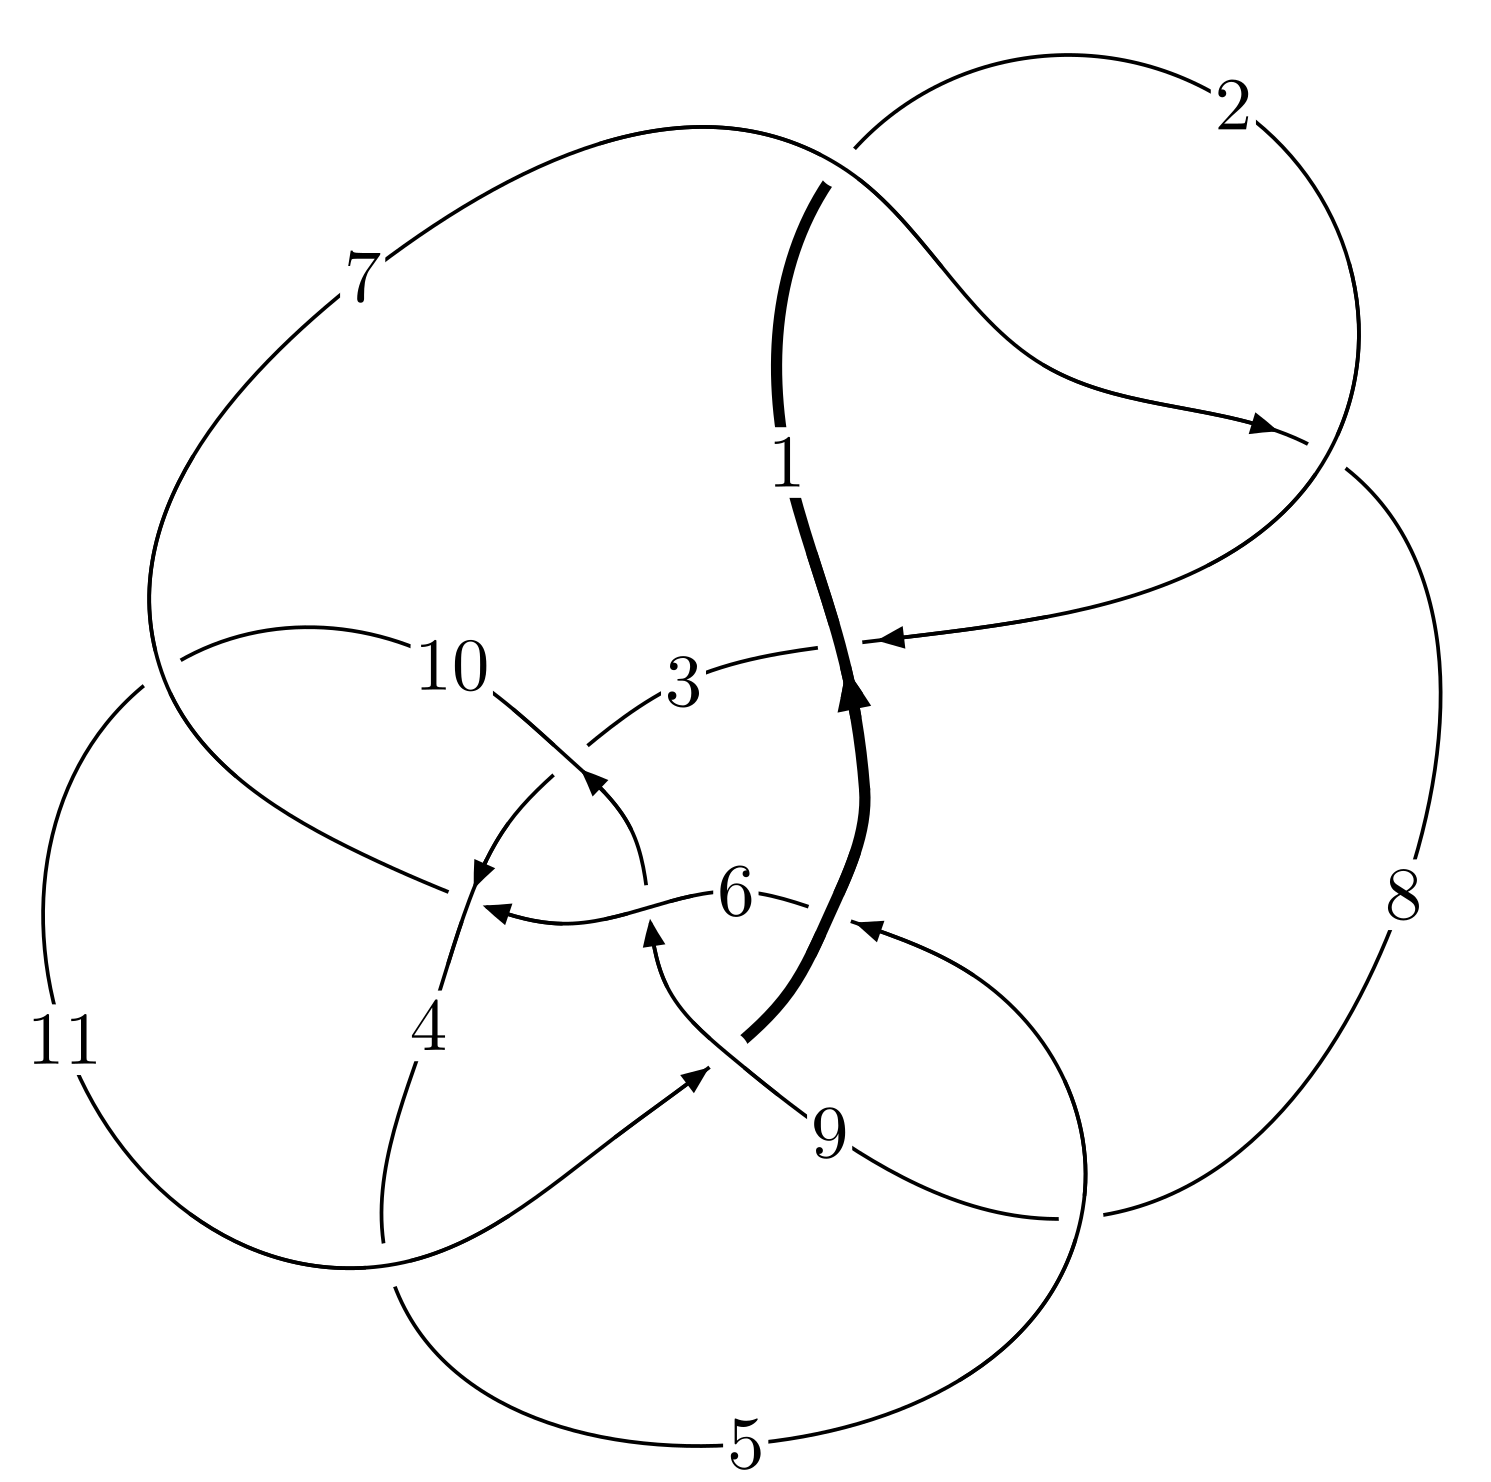
\includegraphics[width=112pt]{../../../GIT/diagram.site/Diagrams/png/764_11n_148.png}\\
\ \ \ A knot diagram\footnotemark}&
\allowdisplaybreaks
\textbf{Linearized knot diagam} \\
\cline{2-2}
 &
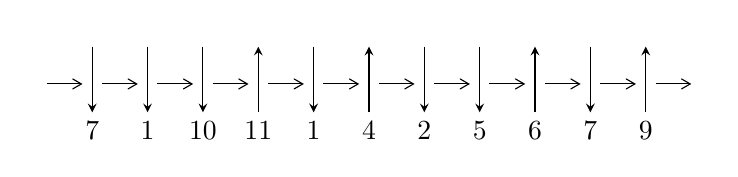
\begin{tikzpicture}[x=20pt, y=17pt]
	% nodes
	\node (C0) at (0, 0) {};
	\node (C1) at (1, 0) {};
	\node (C1U) at (1, +1) {};
	\node (C1D) at (1, -1) {7};

	\node (C2) at (2, 0) {};
	\node (C2U) at (2, +1) {};
	\node (C2D) at (2, -1) {1};

	\node (C3) at (3, 0) {};
	\node (C3U) at (3, +1) {};
	\node (C3D) at (3, -1) {10};

	\node (C4) at (4, 0) {};
	\node (C4U) at (4, +1) {};
	\node (C4D) at (4, -1) {11};

	\node (C5) at (5, 0) {};
	\node (C5U) at (5, +1) {};
	\node (C5D) at (5, -1) {1};

	\node (C6) at (6, 0) {};
	\node (C6U) at (6, +1) {};
	\node (C6D) at (6, -1) {4};

	\node (C7) at (7, 0) {};
	\node (C7U) at (7, +1) {};
	\node (C7D) at (7, -1) {2};

	\node (C8) at (8, 0) {};
	\node (C8U) at (8, +1) {};
	\node (C8D) at (8, -1) {5};

	\node (C9) at (9, 0) {};
	\node (C9U) at (9, +1) {};
	\node (C9D) at (9, -1) {6};

	\node (C10) at (10, 0) {};
	\node (C10U) at (10, +1) {};
	\node (C10D) at (10, -1) {7};

	\node (C11) at (11, 0) {};
	\node (C11U) at (11, +1) {};
	\node (C11D) at (11, -1) {9};
	\node (C12) at (12, 0) {};

	% arrows
	\draw[->,>={angle 60}]
	(C0) edge (C1) (C1) edge (C2) (C2) edge (C3) (C3) edge (C4) (C4) edge (C5) (C5) edge (C6) (C6) edge (C7) (C7) edge (C8) (C8) edge (C9) (C9) edge (C10) (C10) edge (C11) (C11) edge (C12) ;	\draw[->,>=stealth]
	(C1U) edge (C1D) (C2U) edge (C2D) (C3U) edge (C3D) (C4D) edge (C4U) (C5U) edge (C5D) (C6D) edge (C6U) (C7U) edge (C7D) (C8U) edge (C8D) (C9D) edge (C9U) (C10U) edge (C10D) (C11D) edge (C11U) ;
	\end{tikzpicture} \\
\hhline{~~} \\& 
\textbf{Solving Sequence} \\ \cline{2-2} 
 &
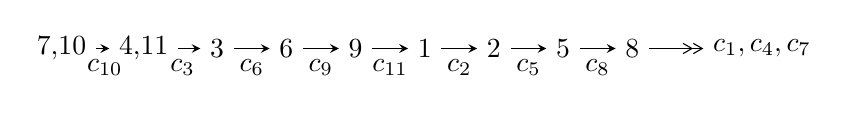
\begin{tikzpicture}[x=25pt, y=7pt]
	% node
	\node (A0) at (-1/8, 0) {7,10};
	\node (A1) at (17/16, 0) {4,11};
	\node (A2) at (17/8, 0) {3};
	\node (A3) at (25/8, 0) {6};
	\node (A4) at (33/8, 0) {9};
	\node (A5) at (41/8, 0) {1};
	\node (A6) at (49/8, 0) {2};
	\node (A7) at (57/8, 0) {5};
	\node (A8) at (65/8, 0) {8};
	\node (C1) at (1/2, -1) {$c_{10}$};
	\node (C2) at (13/8, -1) {$c_{3}$};
	\node (C3) at (21/8, -1) {$c_{6}$};
	\node (C4) at (29/8, -1) {$c_{9}$};
	\node (C5) at (37/8, -1) {$c_{11}$};
	\node (C6) at (45/8, -1) {$c_{2}$};
	\node (C7) at (53/8, -1) {$c_{5}$};
	\node (C8) at (61/8, -1) {$c_{8}$};
	\node (A9) at (10, 0) {$c_{1},c_{4},c_{7}$};

	% edge
	\draw[->,>=stealth]	
	(A0) edge (A1) (A1) edge (A2) (A2) edge (A3) (A3) edge (A4) (A4) edge (A5) (A5) edge (A6) (A6) edge (A7) (A7) edge (A8) ;
	\draw[->>,>={angle 60}]	
	(A8) edge (A9);
\end{tikzpicture} \\ 

\end{tabular} \\

\footnotetext{
The image of knot diagram is generated by the software ``\textbf{Draw programme}" developed by Andrew Bartholomew(\url{http://www.layer8.co.uk/maths/draw/index.htm\#Running-draw}), where we modified some parts for our purpose(\url{https://github.com/CATsTAILs/LinksPainter}).
}\phantom \\ \newline 
\centering \textbf{Ideals for irreducible components\footnotemark of $X_{\text{par}}$} 
 
\begin{align*}
I^u_{1}&=\langle 
b- u,\;3936 u^{12}-3615 u^{11}+\cdots+1546 a+3493,\\
\phantom{I^u_{1}}&\phantom{= \langle  }u^{13}- u^{12}-6 u^{11}+8 u^{10}+21 u^9-27 u^8-41 u^7+43 u^6+41 u^5-35 u^4-12 u^3+10 u^2+u-1\rangle \\
I^u_{2}&=\langle 
b- u,\;-689759 u^{11}-107599 u^{10}+\cdots+501166 a-3895672,\\
\phantom{I^u_{2}}&\phantom{= \langle  }u^{12}- u^{10}+4 u^8-8 u^7+14 u^6+15 u^5-33 u^4+u^3+26 u^2+3 u+1\rangle \\
I^u_{3}&=\langle 
b+u,\;-280773 u^{15}+187752 u^{14}+\cdots+478966 a-1154354,\\
\phantom{I^u_{3}}&\phantom{= \langle  }u^{16}- u^{15}+5 u^{14}-7 u^{13}+8 u^{12}-15 u^{11}+8 u^{10}-6 u^9+11 u^8+10 u^7+11 u^5-4 u^4-5 u^3+u^2+u+1\rangle \\
I^u_{4}&=\langle 
-5 u^7-11 u^6+19 u^4-32 u^3-9 u^2+16 b+41 u+18,\\
\phantom{I^u_{4}}&\phantom{= \langle  }- u^7+5 u^6+12 u^5+3 u^4-20 u^3+55 u^2+32 a-31 u+2,\;u^8+u^7-2 u^6-3 u^5+10 u^4-7 u^3-3 u^2+4\rangle \\
I^u_{5}&=\langle 
1632242669 u^{15}-3999460410 u^{14}+\cdots+68858688392 b+15730031303,\\
\phantom{I^u_{5}}&\phantom{= \langle  }-1552686477 u^{15}+2916463782 u^{14}+\cdots+57539451944 a-28248685713,\\
\phantom{I^u_{5}}&\phantom{= \langle  }u^{16}- u^{15}+\cdots+14 u+61\rangle \\
I^u_{6}&=\langle 
b+u,\;a- u,\;u^2+u+1\rangle \\
I^u_{7}&=\langle 
b- u,\;a,\;u^2+u-1\rangle \\
I^u_{8}&=\langle 
u^3-2 u^2+b-1,\;u^3- u^2+a-2 u-2,\;u^4- u^3-2 u^2-2 u-1\rangle \\
\\
\end{align*}
\raggedright * 8 irreducible components of $\dim_{\mathbb{C}}=0$, with total 73 representations.\\
\footnotetext{All coefficients of polynomials are rational numbers. But the coefficients are sometimes approximated in decimal forms when there is not enough margin.}
\newpage
\renewcommand{\arraystretch}{1}
\centering \section*{I. $I^u_{1}= \langle b- u,\;3936 u^{12}-3615 u^{11}+\cdots+1546 a+3493,\;u^{13}- u^{12}+\cdots+u-1 \rangle$}
\flushleft \textbf{(i) Arc colorings}\\
\begin{tabular}{m{7pt} m{180pt} m{7pt} m{180pt} }
\flushright $a_{7}=$&$\begin{pmatrix}0\\u\end{pmatrix}$ \\
\flushright $a_{10}=$&$\begin{pmatrix}1\\0\end{pmatrix}$ \\
\flushright $a_{4}=$&$\begin{pmatrix}-2.54592 u^{12}+2.33829 u^{11}+\cdots-14.3182 u-2.25938\\u\end{pmatrix}$ \\
\flushright $a_{11}=$&$\begin{pmatrix}1\\u^2\end{pmatrix}$ \\
\flushright $a_{3}=$&$\begin{pmatrix}-2.54592 u^{12}+2.33829 u^{11}+\cdots-13.3182 u-2.25938\\u\end{pmatrix}$ \\
\flushright $a_{6}=$&$\begin{pmatrix}-3.90815 u^{12}+3.32342 u^{11}+\cdots-14.3635 u-2.48124\\0.206339 u^{12}-0.195990 u^{11}+\cdots+3.33829 u+0.207633\end{pmatrix}$ \\
\flushright $a_{9}=$&$\begin{pmatrix}-1.25938 u^{12}-0.286546 u^{11}+\cdots+5.28008 u-6.57762\\- u^2+1\end{pmatrix}$ \\
\flushright $a_{1}=$&$\begin{pmatrix}0.429495 u^{12}+1.13907 u^{11}+\cdots-10.4463 u+3.81307\\-0.197283 u^{12}+0.0588616 u^{11}+\cdots+0.287840 u-2.33959\end{pmatrix}$ \\
\flushright $a_{2}=$&$\begin{pmatrix}0.429495 u^{12}+1.13907 u^{11}+\cdots-10.4463 u+3.81307\\0.190168 u^{12}+0.120310 u^{11}+\cdots-0.851229 u-0.771022\end{pmatrix}$ \\
\flushright $a_{5}=$&$\begin{pmatrix}-2.33959 u^{12}+2.14230 u^{11}+\cdots-10.9799 u-2.05175\\0.0679172 u^{12}-0.0284605 u^{11}+\cdots+1.19599 u+0.0103493\end{pmatrix}$ \\
\flushright $a_{8}=$&$\begin{pmatrix}-1.06210 u^{12}-0.345408 u^{11}+\cdots+4.99224 u-4.23803\\-0.0394567 u^{12}-0.188228 u^{11}+\cdots+0.0575679 u+0.932083\end{pmatrix}$\\ \flushright $a_{8}=$&$\begin{pmatrix}-1.06210 u^{12}-0.345408 u^{11}+\cdots+4.99224 u-4.23803\\-0.0394567 u^{12}-0.188228 u^{11}+\cdots+0.0575679 u+0.932083\end{pmatrix}$\\&\end{tabular}
\flushleft \textbf{(ii) Obstruction class $= -1$}\\~\\
\flushleft \textbf{(iii) Cusp Shapes $= -\frac{5825}{773} u^{12}+\frac{3398}{773} u^{11}+\frac{36475}{773} u^{10}-\frac{31741}{773} u^9-\frac{135781}{773} u^8+\frac{103033}{773} u^7+\frac{280491}{773} u^6-\frac{140065}{773} u^5-\frac{289681}{773} u^4+\frac{91807}{773} u^3+\frac{95194}{773} u^2-\frac{21889}{773} u-\frac{11636}{773}$}\\~\\
\newpage\renewcommand{\arraystretch}{1}
\flushleft \textbf{(iv) u-Polynomials at the component}\newline \\
\begin{tabular}{m{50pt}|m{274pt}}
Crossings & \hspace{64pt}u-Polynomials at each crossing \\
\hline $$\begin{aligned}c_{1},c_{7}\end{aligned}$$&$\begin{aligned}
&u^{13}-6 u^{12}+\cdots-20 u+8
\end{aligned}$\\
\hline $$\begin{aligned}c_{2}\end{aligned}$$&$\begin{aligned}
&u^{13}+10 u^{12}+\cdots+208 u+64
\end{aligned}$\\
\hline $$\begin{aligned}c_{3},c_{5},c_{8}\\c_{10}\end{aligned}$$&$\begin{aligned}
&u^{13}+u^{12}+\cdots+u+1
\end{aligned}$\\
\hline $$\begin{aligned}c_{4},c_{9}\end{aligned}$$&$\begin{aligned}
&u^{13}-2 u^{12}+\cdots- u+4
\end{aligned}$\\
\hline $$\begin{aligned}c_{6},c_{11}\end{aligned}$$&$\begin{aligned}
&u^{13}+5 u^{12}+\cdots+11 u-1
\end{aligned}$\\
\hline
\end{tabular}\\~\\
\newpage\renewcommand{\arraystretch}{1}
\flushleft \textbf{(v) Riley Polynomials at the component}\newline \\
\begin{tabular}{m{50pt}|m{274pt}}
Crossings & \hspace{64pt}Riley Polynomials at each crossing \\
\hline $$\begin{aligned}c_{1},c_{7}\end{aligned}$$&$\begin{aligned}
&y^{13}-10 y^{12}+\cdots+208 y-64
\end{aligned}$\\
\hline $$\begin{aligned}c_{2}\end{aligned}$$&$\begin{aligned}
&y^{13}-14 y^{12}+\cdots-14080 y-4096
\end{aligned}$\\
\hline $$\begin{aligned}c_{3},c_{5},c_{8}\\c_{10}\end{aligned}$$&$\begin{aligned}
&y^{13}-13 y^{12}+\cdots+21 y-1
\end{aligned}$\\
\hline $$\begin{aligned}c_{4},c_{9}\end{aligned}$$&$\begin{aligned}
&y^{13}+16 y^{11}+\cdots+65 y-16
\end{aligned}$\\
\hline $$\begin{aligned}c_{6},c_{11}\end{aligned}$$&$\begin{aligned}
&y^{13}-5 y^{12}+\cdots+157 y-1
\end{aligned}$\\
\hline
\end{tabular}\\~\\
\newpage\flushleft \textbf{(vi) Complex Volumes and Cusp Shapes}
$$\begin{array}{c|c|c}  
\text{Solutions to }I^u_{1}& \I (\text{vol} + \sqrt{-1}CS) & \text{Cusp shape}\\
 \hline 
\begin{aligned}
u &= \phantom{-}0.679240\phantom{ +0.000000I} \\
a &= -0.118511\phantom{ +0.000000I} \\
b &= \phantom{-}0.679240\phantom{ +0.000000I}\end{aligned}
 & -0.985814\phantom{ +0.000000I} & -9.93790\phantom{ +0.000000I} \\ \hline\begin{aligned}
u &= \phantom{-}1.319410 + 0.222030 I \\
a &= \phantom{-}0.746615 - 0.655764 I \\
b &= \phantom{-}1.319410 + 0.222030 I\end{aligned}
 & -1.44982 - 2.92540 I & -5.79046 + 3.21859 I \\ \hline\begin{aligned}
u &= \phantom{-}1.319410 - 0.222030 I \\
a &= \phantom{-}0.746615 + 0.655764 I \\
b &= \phantom{-}1.319410 - 0.222030 I\end{aligned}
 & -1.44982 + 2.92540 I & -5.79046 - 3.21859 I \\ \hline\begin{aligned}
u &= -1.310050 + 0.430816 I \\
a &= -0.729761 + 0.359278 I \\
b &= -1.310050 + 0.430816 I\end{aligned}
 & -9.72048 + 1.68662 I & -6.99569 + 0.12715 I \\ \hline\begin{aligned}
u &= -1.310050 - 0.430816 I \\
a &= -0.729761 - 0.359278 I \\
b &= -1.310050 - 0.430816 I\end{aligned}
 & -9.72048 - 1.68662 I & -6.99569 - 0.12715 I \\ \hline\begin{aligned}
u &= \phantom{-}0.440196 + 0.153722 I \\
a &= -1.05333 + 2.17650 I \\
b &= \phantom{-}0.440196 + 0.153722 I\end{aligned}
 & \phantom{-}0.31710 - 4.56636 I & -5.37309 + 4.90464 I \\ \hline\begin{aligned}
u &= \phantom{-}0.440196 - 0.153722 I \\
a &= -1.05333 - 2.17650 I \\
b &= \phantom{-}0.440196 - 0.153722 I\end{aligned}
 & \phantom{-}0.31710 + 4.56636 I & -5.37309 - 4.90464 I \\ \hline\begin{aligned}
u &= -0.458477 + 0.058416 I \\
a &= \phantom{-}1.85684 + 0.90881 I \\
b &= -0.458477 + 0.058416 I\end{aligned}
 & \phantom{-}2.02562 + 0.48569 I & \phantom{-}2.64958 + 0.42406 I \\ \hline\begin{aligned}
u &= -0.458477 - 0.058416 I \\
a &= \phantom{-}1.85684 - 0.90881 I \\
b &= -0.458477 - 0.058416 I\end{aligned}
 & \phantom{-}2.02562 - 0.48569 I & \phantom{-}2.64958 - 0.42406 I \\ \hline\begin{aligned}
u &= -1.40672 + 0.68037 I \\
a &= -0.434994 - 0.837741 I \\
b &= -1.40672 + 0.68037 I\end{aligned}
 & -1.01550 + 9.99038 I & -3.69502 - 7.61192 I\\
 \hline 
 \end{array}$$\newpage$$\begin{array}{c|c|c}  
\text{Solutions to }I^u_{1}& \I (\text{vol} + \sqrt{-1}CS) & \text{Cusp shape}\\
 \hline 
\begin{aligned}
u &= -1.40672 - 0.68037 I \\
a &= -0.434994 + 0.837741 I \\
b &= -1.40672 - 0.68037 I\end{aligned}
 & -1.01550 - 9.99038 I & -3.69502 + 7.61192 I \\ \hline\begin{aligned}
u &= \phantom{-}1.57602 + 1.15308 I \\
a &= \phantom{-}0.173888 - 0.741516 I \\
b &= \phantom{-}1.57602 + 1.15308 I\end{aligned}
 & -8.5808 - 15.4617 I & -4.82638 + 7.62465 I \\ \hline\begin{aligned}
u &= \phantom{-}1.57602 - 1.15308 I \\
a &= \phantom{-}0.173888 + 0.741516 I \\
b &= \phantom{-}1.57602 - 1.15308 I\end{aligned}
 & -8.5808 + 15.4617 I & -4.82638 - 7.62465 I\\
 \hline 
 \end{array}$$\newpage\newpage\renewcommand{\arraystretch}{1}
\centering \section*{II. $I^u_{2}= \langle b- u,\;-6.90\times10^{5} u^{11}-1.08\times10^{5} u^{10}+\cdots+5.01\times10^{5} a-3.90\times10^{6},\;u^{12}- u^{10}+\cdots+3 u+1 \rangle$}
\flushleft \textbf{(i) Arc colorings}\\
\begin{tabular}{m{7pt} m{180pt} m{7pt} m{180pt} }
\flushright $a_{7}=$&$\begin{pmatrix}0\\u\end{pmatrix}$ \\
\flushright $a_{10}=$&$\begin{pmatrix}1\\0\end{pmatrix}$ \\
\flushright $a_{4}=$&$\begin{pmatrix}1.37631 u^{11}+0.214697 u^{10}+\cdots+42.8501 u+7.77322\\u\end{pmatrix}$ \\
\flushright $a_{11}=$&$\begin{pmatrix}1\\u^2\end{pmatrix}$ \\
\flushright $a_{3}=$&$\begin{pmatrix}1.37631 u^{11}+0.214697 u^{10}+\cdots+43.8501 u+7.77322\\u\end{pmatrix}$ \\
\flushright $a_{6}=$&$\begin{pmatrix}2.34713 u^{11}+0.345161 u^{10}+\cdots+61.9493 u+17.9990\\0.209352 u^{11}-0.148428 u^{10}+\cdots+3.02040 u+0.214697\end{pmatrix}$ \\
\flushright $a_{9}=$&$\begin{pmatrix}1.45089 u^{11}-0.0821125 u^{10}+\cdots+40.5075 u-3.80051\\-0.0710822 u^{11}+0.0690011 u^{10}+\cdots-0.602275 u-0.458944\end{pmatrix}$ \\
\flushright $a_{1}=$&$\begin{pmatrix}1.03465 u^{11}+0.0271287 u^{10}+\cdots+28.9476 u-0.912330\\0.0773456 u^{11}+0.0652877 u^{10}+\cdots-0.188917 u-0.249592\end{pmatrix}$ \\
\flushright $a_{2}=$&$\begin{pmatrix}1.03465 u^{11}+0.0271287 u^{10}+\cdots+28.9476 u-0.912330\\0.0341124 u^{11}+0.224690 u^{10}+\cdots-1.30495 u-0.276721\end{pmatrix}$ \\
\flushright $a_{5}=$&$\begin{pmatrix}1.58566 u^{11}+0.0662695 u^{10}+\cdots+45.8705 u+7.98791\\0.00371334 u^{11}-0.251541 u^{10}+\cdots+1.23593 u+0.148428\end{pmatrix}$ \\
\flushright $a_{8}=$&$\begin{pmatrix}-0.708286 u^{11}+0.253305 u^{10}+\cdots-15.0153 u+5.51408\\-0.251541 u^{11}-0.0941345 u^{10}+\cdots+0.137288 u-0.00371334\end{pmatrix}$\\ \flushright $a_{8}=$&$\begin{pmatrix}-0.708286 u^{11}+0.253305 u^{10}+\cdots-15.0153 u+5.51408\\-0.251541 u^{11}-0.0941345 u^{10}+\cdots+0.137288 u-0.00371334\end{pmatrix}$\\&\end{tabular}
\flushleft \textbf{(ii) Obstruction class $= -1$}\\~\\
\flushleft \textbf{(iii) Cusp Shapes $= \frac{2218099}{501166} u^{11}-\frac{163295}{250583} u^{10}+\cdots+\frac{55914373}{501166} u-\frac{2178981}{501166}$}\\~\\
\newpage\renewcommand{\arraystretch}{1}
\flushleft \textbf{(iv) u-Polynomials at the component}\newline \\
\begin{tabular}{m{50pt}|m{274pt}}
Crossings & \hspace{64pt}u-Polynomials at each crossing \\
\hline $$\begin{aligned}c_{1},c_{7}\end{aligned}$$&$\begin{aligned}
&(u^6-4 u^5+6 u^4-5 u^3+5 u^2-6 u+4)^2
\end{aligned}$\\
\hline $$\begin{aligned}c_{2}\end{aligned}$$&$\begin{aligned}
&(u^6+4 u^5+6 u^4+5 u^3+13 u^2-4 u+16)^2
\end{aligned}$\\
\hline $$\begin{aligned}c_{3},c_{5},c_{8}\\c_{10}\end{aligned}$$&$\begin{aligned}
&u^{12}- u^{10}+4 u^8+8 u^7+14 u^6-15 u^5-33 u^4- u^3+26 u^2-3 u+1
\end{aligned}$\\
\hline $$\begin{aligned}c_{4},c_{9}\end{aligned}$$&$\begin{aligned}
&(u^6+u^5+3 u^4+u^3+4 u^2+1)^2
\end{aligned}$\\
\hline $$\begin{aligned}c_{6},c_{11}\end{aligned}$$&$\begin{aligned}
&u^{12}+4 u^{11}+\cdots+66 u+11
\end{aligned}$\\
\hline
\end{tabular}\\~\\
\newpage\renewcommand{\arraystretch}{1}
\flushleft \textbf{(v) Riley Polynomials at the component}\newline \\
\begin{tabular}{m{50pt}|m{274pt}}
Crossings & \hspace{64pt}Riley Polynomials at each crossing \\
\hline $$\begin{aligned}c_{1},c_{7}\end{aligned}$$&$\begin{aligned}
&(y^6-4 y^5+6 y^4-5 y^3+13 y^2+4 y+16)^2
\end{aligned}$\\
\hline $$\begin{aligned}c_{2}\end{aligned}$$&$\begin{aligned}
&(y^6-4 y^5+22 y^4+195 y^3+401 y^2+400 y+256)^2
\end{aligned}$\\
\hline $$\begin{aligned}c_{3},c_{5},c_{8}\\c_{10}\end{aligned}$$&$\begin{aligned}
&y^{12}-2 y^{11}+\cdots+43 y+1
\end{aligned}$\\
\hline $$\begin{aligned}c_{4},c_{9}\end{aligned}$$&$\begin{aligned}
&(y^6+5 y^5+15 y^4+25 y^3+22 y^2+8 y+1)^2
\end{aligned}$\\
\hline $$\begin{aligned}c_{6},c_{11}\end{aligned}$$&$\begin{aligned}
&y^{12}-4 y^{11}+\cdots-484 y+121
\end{aligned}$\\
\hline
\end{tabular}\\~\\
\newpage\flushleft \textbf{(vi) Complex Volumes and Cusp Shapes}
$$\begin{array}{c|c|c}  
\text{Solutions to }I^u_{2}& \I (\text{vol} + \sqrt{-1}CS) & \text{Cusp shape}\\
 \hline 
\begin{aligned}
u &= -0.968045 + 0.076481 I \\
a &= -0.541139 - 1.217710 I \\
b &= -0.968045 + 0.076481 I\end{aligned}
 & -2.70944 - 2.74874 I & -6.55410 + 3.66193 I \\ \hline\begin{aligned}
u &= -0.968045 - 0.076481 I \\
a &= -0.541139 + 1.217710 I \\
b &= -0.968045 - 0.076481 I\end{aligned}
 & -2.70944 + 2.74874 I & -6.55410 - 3.66193 I \\ \hline\begin{aligned}
u &= \phantom{-}1.126210 + 0.587419 I \\
a &= \phantom{-}1.063370 + 0.516394 I \\
b &= \phantom{-}1.126210 + 0.587419 I\end{aligned}
 & -9.45817 - 7.70670 I & -6.10501 + 5.38862 I \\ \hline\begin{aligned}
u &= \phantom{-}1.126210 - 0.587419 I \\
a &= \phantom{-}1.063370 - 0.516394 I \\
b &= \phantom{-}1.126210 - 0.587419 I\end{aligned}
 & -9.45817 + 7.70670 I & -6.10501 - 5.38862 I \\ \hline\begin{aligned}
u &= \phantom{-}1.176980 + 0.755737 I \\
a &= \phantom{-}0.136599 - 0.758615 I \\
b &= \phantom{-}1.176980 + 0.755737 I\end{aligned}
 & -2.70944 - 2.74874 I & -6.55410 + 3.66193 I \\ \hline\begin{aligned}
u &= \phantom{-}1.176980 - 0.755737 I \\
a &= \phantom{-}0.136599 + 0.758615 I \\
b &= \phantom{-}1.176980 - 0.755737 I\end{aligned}
 & -2.70944 + 2.74874 I & -6.55410 - 3.66193 I \\ \hline\begin{aligned}
u &= \phantom{-}0.19389 + 1.60136 I \\
a &= \phantom{-}0.007131 - 0.411898 I \\
b &= \phantom{-}0.19389 + 1.60136 I\end{aligned}
 & \phantom{-}3.94294 - 2.97593 I & -11.8409 + 20.9878 I \\ \hline\begin{aligned}
u &= \phantom{-}0.19389 - 1.60136 I \\
a &= \phantom{-}0.007131 + 0.411898 I \\
b &= \phantom{-}0.19389 - 1.60136 I\end{aligned}
 & \phantom{-}3.94294 + 2.97593 I & -11.8409 - 20.9878 I \\ \hline\begin{aligned}
u &= -0.052940 + 0.185549 I \\
a &= \phantom{-}5.45961 + 8.32725 I \\
b &= -0.052940 + 0.185549 I\end{aligned}
 & \phantom{-}3.94294 - 2.97593 I & -11.8409 + 20.9878 I \\ \hline\begin{aligned}
u &= -0.052940 - 0.185549 I \\
a &= \phantom{-}5.45961 - 8.32725 I \\
b &= -0.052940 - 0.185549 I\end{aligned}
 & \phantom{-}3.94294 + 2.97593 I & -11.8409 - 20.9878 I\\
 \hline 
 \end{array}$$\newpage$$\begin{array}{c|c|c}  
\text{Solutions to }I^u_{2}& \I (\text{vol} + \sqrt{-1}CS) & \text{Cusp shape}\\
 \hline 
\begin{aligned}
u &= -1.47610 + 1.13544 I \\
a &= -0.125567 - 0.653945 I \\
b &= -1.47610 + 1.13544 I\end{aligned}
 & -9.45817 + 7.70670 I & -6.10501 - 5.38862 I \\ \hline\begin{aligned}
u &= -1.47610 - 1.13544 I \\
a &= -0.125567 + 0.653945 I \\
b &= -1.47610 - 1.13544 I\end{aligned}
 & -9.45817 - 7.70670 I & -6.10501 + 5.38862 I\\
 \hline 
 \end{array}$$\newpage\newpage\renewcommand{\arraystretch}{1}
\centering \section*{III. $I^u_{3}= \langle b+u,\;-2.81\times10^{5} u^{15}+1.88\times10^{5} u^{14}+\cdots+4.79\times10^{5} a-1.15\times10^{6},\;u^{16}- u^{15}+\cdots+u+1 \rangle$}
\flushleft \textbf{(i) Arc colorings}\\
\begin{tabular}{m{7pt} m{180pt} m{7pt} m{180pt} }
\flushright $a_{7}=$&$\begin{pmatrix}0\\u\end{pmatrix}$ \\
\flushright $a_{10}=$&$\begin{pmatrix}1\\0\end{pmatrix}$ \\
\flushright $a_{4}=$&$\begin{pmatrix}0.586207 u^{15}-0.391994 u^{14}+\cdots+2.99697 u+2.41010\\- u\end{pmatrix}$ \\
\flushright $a_{11}=$&$\begin{pmatrix}1\\u^2\end{pmatrix}$ \\
\flushright $a_{3}=$&$\begin{pmatrix}0.586207 u^{15}-0.391994 u^{14}+\cdots+1.99697 u+2.41010\\- u\end{pmatrix}$ \\
\flushright $a_{6}=$&$\begin{pmatrix}1.60046 u^{15}-1.09856 u^{14}+\cdots+0.905045 u+5.14908\\-0.370010 u^{15}+0.495060 u^{14}+\cdots+0.219581 u-0.194212\end{pmatrix}$ \\
\flushright $a_{9}=$&$\begin{pmatrix}-0.982304 u^{15}+1.65935 u^{14}+\cdots-5.17282 u+0.456744\\0.155410 u^{15}-0.318879 u^{14}+\cdots+0.496238 u+0.382754\end{pmatrix}$ \\
\flushright $a_{1}=$&$\begin{pmatrix}0.459400 u^{15}-0.696398 u^{14}+\cdots+4.05434 u+0.305940\\-0.631821 u^{15}+0.786116 u^{14}+\cdots-0.118524 u-0.511907\end{pmatrix}$ \\
\flushright $a_{2}=$&$\begin{pmatrix}0.459400 u^{15}-0.696398 u^{14}+\cdots+4.05434 u+0.305940\\-0.726319 u^{15}+0.940998 u^{14}+\cdots-0.340926 u-0.274909\end{pmatrix}$ \\
\flushright $a_{5}=$&$\begin{pmatrix}0.956216 u^{15}-0.887055 u^{14}+\cdots+2.77739 u+2.60431\\0.0409340 u^{15}-0.0327789 u^{14}+\cdots-1.24496 u+0.125051\end{pmatrix}$ \\
\flushright $a_{8}=$&$\begin{pmatrix}0.667893 u^{15}-1.05794 u^{14}+\cdots+2.47945 u-1.10540\\0.681729 u^{15}-0.825163 u^{14}+\cdots-0.159324 u+0.901951\end{pmatrix}$\\ \flushright $a_{8}=$&$\begin{pmatrix}0.667893 u^{15}-1.05794 u^{14}+\cdots+2.47945 u-1.10540\\0.681729 u^{15}-0.825163 u^{14}+\cdots-0.159324 u+0.901951\end{pmatrix}$\\&\end{tabular}
\flushleft \textbf{(ii) Obstruction class $= 1$}\\~\\
\flushleft \textbf{(iii) Cusp Shapes $= -\frac{1422603}{239483} u^{15}+\frac{4693355}{478966} u^{14}+\cdots-\frac{9817835}{478966} u+\frac{275497}{478966}$}\\~\\
\newpage\renewcommand{\arraystretch}{1}
\flushleft \textbf{(iv) u-Polynomials at the component}\newline \\
\begin{tabular}{m{50pt}|m{274pt}}
Crossings & \hspace{64pt}u-Polynomials at each crossing \\
\hline $$\begin{aligned}c_{1},c_{7}\end{aligned}$$&$\begin{aligned}
&u^{16}-9 u^{14}+35 u^{12}-82 u^{10}+133 u^8-152 u^6+118 u^4-56 u^2+13
\end{aligned}$\\
\hline $$\begin{aligned}c_{2}\end{aligned}$$&$\begin{aligned}
&(u^8+9 u^7+35 u^6+82 u^5+133 u^4+152 u^3+118 u^2+56 u+13)^2
\end{aligned}$\\
\hline $$\begin{aligned}c_{3},c_{5},c_{8}\\c_{10}\end{aligned}$$&$\begin{aligned}
&u^{16}- u^{15}+\cdots+u+1
\end{aligned}$\\
\hline $$\begin{aligned}c_{4},c_{9}\end{aligned}$$&$\begin{aligned}
&(u^8+u^7- u^5-3 u^4+u^3+4 u^2+u+1)^2
\end{aligned}$\\
\hline $$\begin{aligned}c_{6},c_{11}\end{aligned}$$&$\begin{aligned}
&u^{16}-9 u^{15}+\cdots-6 u+1
\end{aligned}$\\
\hline
\end{tabular}\\~\\
\newpage\renewcommand{\arraystretch}{1}
\flushleft \textbf{(v) Riley Polynomials at the component}\newline \\
\begin{tabular}{m{50pt}|m{274pt}}
Crossings & \hspace{64pt}Riley Polynomials at each crossing \\
\hline $$\begin{aligned}c_{1},c_{7}\end{aligned}$$&$\begin{aligned}
&(y^8-9 y^7+35 y^6-82 y^5+133 y^4-152 y^3+118 y^2-56 y+13)^2
\end{aligned}$\\
\hline $$\begin{aligned}c_{2}\end{aligned}$$&$\begin{aligned}
&(y^8-11 y^7+15 y^6+86 y^5+39 y^4+10 y^3+358 y^2-68 y+169)^2
\end{aligned}$\\
\hline $$\begin{aligned}c_{3},c_{5},c_{8}\\c_{10}\end{aligned}$$&$\begin{aligned}
&y^{16}+9 y^{15}+\cdots+y+1
\end{aligned}$\\
\hline $$\begin{aligned}c_{4},c_{9}\end{aligned}$$&$\begin{aligned}
&(y^8- y^7-4 y^6+5 y^5+11 y^4-23 y^3+8 y^2+7 y+1)^2
\end{aligned}$\\
\hline $$\begin{aligned}c_{6},c_{11}\end{aligned}$$&$\begin{aligned}
&y^{16}-9 y^{15}+\cdots-2 y+1
\end{aligned}$\\
\hline
\end{tabular}\\~\\
\newpage\flushleft \textbf{(vi) Complex Volumes and Cusp Shapes}
$$\begin{array}{c|c|c}  
\text{Solutions to }I^u_{3}& \I (\text{vol} + \sqrt{-1}CS) & \text{Cusp shape}\\
 \hline 
\begin{aligned}
u &= \phantom{-}0.274263 + 1.008870 I \\
a &= \phantom{-}0.79810 + 1.33602 I \\
b &= -0.274263 - 1.008870 I\end{aligned}
 & \phantom{-}1.71914 - 5.38582 I & -0.93122 + 9.75922 I \\ \hline\begin{aligned}
u &= \phantom{-}0.274263 - 1.008870 I \\
a &= \phantom{-}0.79810 - 1.33602 I \\
b &= -0.274263 + 1.008870 I\end{aligned}
 & \phantom{-}1.71914 + 5.38582 I & -0.93122 - 9.75922 I \\ \hline\begin{aligned}
u &= -0.638849 + 1.040850 I \\
a &= -0.169502 + 1.235590 I \\
b &= \phantom{-}0.638849 - 1.040850 I\end{aligned}
 & \phantom{-}2.34546 + 2.94891 I & \phantom{-}0.795967 + 0.602909 I \\ \hline\begin{aligned}
u &= -0.638849 - 1.040850 I \\
a &= -0.169502 - 1.235590 I \\
b &= \phantom{-}0.638849 + 1.040850 I\end{aligned}
 & \phantom{-}2.34546 - 2.94891 I & \phantom{-}0.795967 - 0.602909 I \\ \hline\begin{aligned}
u &= -0.701878 + 0.091386 I \\
a &= -0.850232 - 0.808730 I \\
b &= \phantom{-}0.701878 - 0.091386 I\end{aligned}
 & \phantom{-}1.71914 + 5.38582 I & -0.93122 - 9.75922 I \\ \hline\begin{aligned}
u &= -0.701878 - 0.091386 I \\
a &= -0.850232 + 0.808730 I \\
b &= \phantom{-}0.701878 + 0.091386 I\end{aligned}
 & \phantom{-}1.71914 - 5.38582 I & -0.93122 + 9.75922 I \\ \hline\begin{aligned}
u &= \phantom{-}0.610814 + 0.255978 I \\
a &= \phantom{-}1.098150 - 0.544353 I \\
b &= -0.610814 - 0.255978 I\end{aligned}
 & \phantom{-}2.34546 + 2.94891 I & \phantom{-}0.795967 + 0.602909 I \\ \hline\begin{aligned}
u &= \phantom{-}0.610814 - 0.255978 I \\
a &= \phantom{-}1.098150 + 0.544353 I \\
b &= -0.610814 + 0.255978 I\end{aligned}
 & \phantom{-}2.34546 - 2.94891 I & \phantom{-}0.795967 - 0.602909 I \\ \hline\begin{aligned}
u &= \phantom{-}1.305320 + 0.359264 I \\
a &= -0.481994 + 0.934732 I \\
b &= -1.305320 - 0.359264 I\end{aligned}
 & -6.45579 - 3.75611 I & -8.46169 + 3.08159 I \\ \hline\begin{aligned}
u &= \phantom{-}1.305320 - 0.359264 I \\
a &= -0.481994 - 0.934732 I \\
b &= -1.305320 + 0.359264 I\end{aligned}
 & -6.45579 + 3.75611 I & -8.46169 - 3.08159 I\\
 \hline 
 \end{array}$$\newpage$$\begin{array}{c|c|c}  
\text{Solutions to }I^u_{3}& \I (\text{vol} + \sqrt{-1}CS) & \text{Cusp shape}\\
 \hline 
\begin{aligned}
u &= -0.213253 + 0.417979 I \\
a &= \phantom{-}2.89265 + 2.89484 I \\
b &= \phantom{-}0.213253 - 0.417979 I\end{aligned}
 & \phantom{-}4.03613 - 2.81197 I & \phantom{-}9.0969 - 15.4678 I \\ \hline\begin{aligned}
u &= -0.213253 - 0.417979 I \\
a &= \phantom{-}2.89265 - 2.89484 I \\
b &= \phantom{-}0.213253 + 0.417979 I\end{aligned}
 & \phantom{-}4.03613 + 2.81197 I & \phantom{-}9.0969 + 15.4678 I \\ \hline\begin{aligned}
u &= -0.24620 + 1.56767 I \\
a &= \phantom{-}0.067177 + 0.435558 I \\
b &= \phantom{-}0.24620 - 1.56767 I\end{aligned}
 & \phantom{-}4.03613 + 2.81197 I & \phantom{-}9.0969 + 15.4678 I \\ \hline\begin{aligned}
u &= -0.24620 - 1.56767 I \\
a &= \phantom{-}0.067177 - 0.435558 I \\
b &= \phantom{-}0.24620 + 1.56767 I\end{aligned}
 & \phantom{-}4.03613 - 2.81197 I & \phantom{-}9.0969 - 15.4678 I \\ \hline\begin{aligned}
u &= \phantom{-}0.10979 + 1.65368 I \\
a &= \phantom{-}0.145647 + 0.120240 I \\
b &= -0.10979 - 1.65368 I\end{aligned}
 & -6.45579 - 3.75611 I & -8.46169 + 3.08159 I \\ \hline\begin{aligned}
u &= \phantom{-}0.10979 - 1.65368 I \\
a &= \phantom{-}0.145647 - 0.120240 I \\
b &= -0.10979 + 1.65368 I\end{aligned}
 & -6.45579 + 3.75611 I & -8.46169 - 3.08159 I\\
 \hline 
 \end{array}$$\newpage\newpage\renewcommand{\arraystretch}{1}
\centering \section*{IV. $I^u_{4}= \langle -5 u^7-11 u^6+\cdots+16 b+18,\;- u^7+5 u^6+\cdots+32 a+2,\;u^8+u^7-2 u^6-3 u^5+10 u^4-7 u^3-3 u^2+4 \rangle$}
\flushleft \textbf{(i) Arc colorings}\\
\begin{tabular}{m{7pt} m{180pt} m{7pt} m{180pt} }
\flushright $a_{7}=$&$\begin{pmatrix}0\\u\end{pmatrix}$ \\
\flushright $a_{10}=$&$\begin{pmatrix}1\\0\end{pmatrix}$ \\
\flushright $a_{4}=$&$\begin{pmatrix}0.0312500 u^{7}-0.156250 u^{6}+\cdots+0.968750 u-0.0625000\\\frac{5}{16} u^7+\frac{11}{16} u^6+\cdots-\frac{41}{16} u-\frac{9}{8}\end{pmatrix}$ \\
\flushright $a_{11}=$&$\begin{pmatrix}1\\u^2\end{pmatrix}$ \\
\flushright $a_{3}=$&$\begin{pmatrix}0.343750 u^{7}+0.531250 u^{6}+\cdots-1.59375 u-1.18750\\\frac{5}{16} u^7+\frac{11}{16} u^6+\cdots-\frac{41}{16} u-\frac{9}{8}\end{pmatrix}$ \\
\flushright $a_{6}=$&$\begin{pmatrix}-0.218750 u^{7}-0.406250 u^{6}+\cdots+1.71875 u-0.0625000\\\frac{1}{16} u^7-\frac{1}{16} u^6+\cdots-\frac{5}{16} u+\frac{3}{8}\end{pmatrix}$ \\
\flushright $a_{9}=$&$\begin{pmatrix}0.0937500 u^{7}+0.281250 u^{6}+\cdots-0.343750 u-0.687500\\\frac{5}{16} u^7+\frac{7}{16} u^6+\cdots-\frac{5}{16} u-\frac{5}{8}\end{pmatrix}$ \\
\flushright $a_{1}=$&$\begin{pmatrix}-0.0937500 u^{7}-0.281250 u^{6}+\cdots+0.843750 u+1.18750\\-\frac{5}{16} u^7-\frac{7}{16} u^6+\cdots+\frac{5}{16} u+\frac{13}{8}\end{pmatrix}$ \\
\flushright $a_{2}=$&$\begin{pmatrix}-0.0937500 u^{7}-0.281250 u^{6}+\cdots+0.843750 u+1.18750\\-0.437500 u^{7}-0.562500 u^{6}+\cdots+0.687500 u+2.37500\end{pmatrix}$ \\
\flushright $a_{5}=$&$\begin{pmatrix}0.468750 u^{7}+0.906250 u^{6}+\cdots-1.46875 u-1.93750\\0.812500 u^{7}+1.68750 u^{6}+\cdots-4.31250 u-3.62500\end{pmatrix}$ \\
\flushright $a_{8}=$&$\begin{pmatrix}-0.343750 u^{7}-0.531250 u^{6}+\cdots+1.59375 u+1.18750\\-0.562500 u^{7}-0.937500 u^{6}+\cdots+3.31250 u+2.62500\end{pmatrix}$\\ \flushright $a_{8}=$&$\begin{pmatrix}-0.343750 u^{7}-0.531250 u^{6}+\cdots+1.59375 u+1.18750\\-0.562500 u^{7}-0.937500 u^{6}+\cdots+3.31250 u+2.62500\end{pmatrix}$\\&\end{tabular}
\flushleft \textbf{(ii) Obstruction class $= -1$}\\~\\
\flushleft \textbf{(iii) Cusp Shapes $= -\frac{3}{2} u^7-\frac{5}{2} u^6+\frac{5}{2} u^4-12 u^3+\frac{17}{2} u^2-\frac{1}{2} u-7$}\\~\\
\newpage\renewcommand{\arraystretch}{1}
\flushleft \textbf{(iv) u-Polynomials at the component}\newline \\
\begin{tabular}{m{50pt}|m{274pt}}
Crossings & \hspace{64pt}u-Polynomials at each crossing \\
\hline $$\begin{aligned}c_{1},c_{7}\end{aligned}$$&$\begin{aligned}
&(u^2+u-1)^4
\end{aligned}$\\
\hline $$\begin{aligned}c_{2}\end{aligned}$$&$\begin{aligned}
&(u^2+3 u+1)^4
\end{aligned}$\\
\hline $$\begin{aligned}c_{3},c_{5},c_{8}\\c_{10}\end{aligned}$$&$\begin{aligned}
&u^8- u^7-2 u^6+3 u^5+10 u^4+7 u^3-3 u^2+4
\end{aligned}$\\
\hline $$\begin{aligned}c_{4},c_{9}\end{aligned}$$&$\begin{aligned}
&u^8-3 u^7+8 u^6-3 u^5+8 u^4-3 u^3+7 u^2+16
\end{aligned}$\\
\hline $$\begin{aligned}c_{6},c_{11}\end{aligned}$$&$\begin{aligned}
&(u^2- u+1)^4
\end{aligned}$\\
\hline
\end{tabular}\\~\\
\newpage\renewcommand{\arraystretch}{1}
\flushleft \textbf{(v) Riley Polynomials at the component}\newline \\
\begin{tabular}{m{50pt}|m{274pt}}
Crossings & \hspace{64pt}Riley Polynomials at each crossing \\
\hline $$\begin{aligned}c_{1},c_{7}\end{aligned}$$&$\begin{aligned}
&(y^2-3 y+1)^4
\end{aligned}$\\
\hline $$\begin{aligned}c_{2}\end{aligned}$$&$\begin{aligned}
&(y^2-7 y+1)^4
\end{aligned}$\\
\hline $$\begin{aligned}c_{3},c_{5},c_{8}\\c_{10}\end{aligned}$$&$\begin{aligned}
&y^8-5 y^7+30 y^6-41 y^5+78 y^4-125 y^3+89 y^2-24 y+16
\end{aligned}$\\
\hline $$\begin{aligned}c_{4},c_{9}\end{aligned}$$&$\begin{aligned}
&y^8+7 y^7+62 y^6+115 y^5+190 y^4+359 y^3+305 y^2+224 y+256
\end{aligned}$\\
\hline $$\begin{aligned}c_{6},c_{11}\end{aligned}$$&$\begin{aligned}
&(y^2+y+1)^4
\end{aligned}$\\
\hline
\end{tabular}\\~\\
\newpage\flushleft \textbf{(vi) Complex Volumes and Cusp Shapes}
$$\begin{array}{c|c|c}  
\text{Solutions to }I^u_{4}& \I (\text{vol} + \sqrt{-1}CS) & \text{Cusp shape}\\
 \hline 
\begin{aligned}
u &= \phantom{-}1.024520 + 0.199293 I \\
a &= -0.628676 - 0.723008 I \\
b &= -1.83354 + 1.20197 I\end{aligned}
 & -8.88264 + 4.05977 I & -10.00000 - 6.92820 I \\ \hline\begin{aligned}
u &= \phantom{-}1.024520 - 0.199293 I \\
a &= -0.628676 + 0.723008 I \\
b &= -1.83354 - 1.20197 I\end{aligned}
 & -8.88264 - 4.05977 I & -10.00000 + 6.92820 I \\ \hline\begin{aligned}
u &= \phantom{-}0.785903 + 1.018910 I \\
a &= \phantom{-}0.295593 + 0.718718 I \\
b &= -0.476886 - 0.483675 I\end{aligned}
 & -0.98696 - 4.05977 I & -10.00000 + 6.92820 I \\ \hline\begin{aligned}
u &= \phantom{-}0.785903 - 1.018910 I \\
a &= \phantom{-}0.295593 - 0.718718 I \\
b &= -0.476886 + 0.483675 I\end{aligned}
 & -0.98696 + 4.05977 I & -10.00000 - 6.92820 I \\ \hline\begin{aligned}
u &= -0.476886 + 0.483675 I \\
a &= -0.39108 + 1.41935 I \\
b &= \phantom{-}0.785903 - 1.018910 I\end{aligned}
 & -0.98696 + 4.05977 I & -10.00000 - 6.92820 I \\ \hline\begin{aligned}
u &= -0.476886 - 0.483675 I \\
a &= -0.39108 - 1.41935 I \\
b &= \phantom{-}0.785903 + 1.018910 I\end{aligned}
 & -0.98696 - 4.05977 I & -10.00000 + 6.92820 I \\ \hline\begin{aligned}
u &= -1.83354 + 1.20197 I \\
a &= -0.025832 + 0.455391 I \\
b &= \phantom{-}1.024520 + 0.199293 I\end{aligned}
 & -8.88264 + 4.05977 I & -10.00000 - 6.92820 I \\ \hline\begin{aligned}
u &= -1.83354 - 1.20197 I \\
a &= -0.025832 - 0.455391 I \\
b &= \phantom{-}1.024520 - 0.199293 I\end{aligned}
 & -8.88264 - 4.05977 I & -10.00000 + 6.92820 I\\
 \hline 
 \end{array}$$\newpage\newpage\renewcommand{\arraystretch}{1}
\centering \section*{V. $I^u_{5}= \langle 1.63\times10^{9} u^{15}-4.00\times10^{9} u^{14}+\cdots+6.89\times10^{10} b+1.57\times10^{10},\;-1.55\times10^{9} u^{15}+2.92\times10^{9} u^{14}+\cdots+5.75\times10^{10} a-2.82\times10^{10},\;u^{16}- u^{15}+\cdots+14 u+61 \rangle$}
\flushleft \textbf{(i) Arc colorings}\\
\begin{tabular}{m{7pt} m{180pt} m{7pt} m{180pt} }
\flushright $a_{7}=$&$\begin{pmatrix}0\\u\end{pmatrix}$ \\
\flushright $a_{10}=$&$\begin{pmatrix}1\\0\end{pmatrix}$ \\
\flushright $a_{4}=$&$\begin{pmatrix}0.0269847 u^{15}-0.0506863 u^{14}+\cdots+0.983334 u+0.490945\\-0.0237042 u^{15}+0.0580821 u^{14}+\cdots-0.637455 u-0.228439\end{pmatrix}$ \\
\flushright $a_{11}=$&$\begin{pmatrix}1\\u^2\end{pmatrix}$ \\
\flushright $a_{3}=$&$\begin{pmatrix}0.00328049 u^{15}+0.00739581 u^{14}+\cdots+0.345879 u+0.262505\\-0.0237042 u^{15}+0.0580821 u^{14}+\cdots-0.637455 u-0.228439\end{pmatrix}$ \\
\flushright $a_{6}=$&$\begin{pmatrix}0.0153528 u^{15}-0.0613303 u^{14}+\cdots+2.50796 u-1.49414\\-0.0137597 u^{15}+0.0519593 u^{14}+\cdots-0.953981 u+0.952940\end{pmatrix}$ \\
\flushright $a_{9}=$&$\begin{pmatrix}0.0119361 u^{15}-0.0470317 u^{14}+\cdots+1.26128 u-0.453422\\0.0267082 u^{15}-0.0380007 u^{14}+\cdots+0.241699 u+1.87605\end{pmatrix}$ \\
\flushright $a_{1}=$&$\begin{pmatrix}0.0131130 u^{15}-0.0237893 u^{14}+\cdots+0.375432 u-0.0329971\\-0.0392634 u^{15}+0.0682124 u^{14}+\cdots-0.0372592 u-1.55608\end{pmatrix}$ \\
\flushright $a_{2}=$&$\begin{pmatrix}0.0131130 u^{15}-0.0237893 u^{14}+\cdots+0.375432 u-0.0329971\\-0.0376838 u^{15}+0.0837224 u^{14}+\cdots-0.687681 u-0.904829\end{pmatrix}$ \\
\flushright $a_{5}=$&$\begin{pmatrix}0.0137569 u^{15}-0.0478038 u^{14}+\cdots+1.66013 u-1.18329\\0.0333257 u^{15}-0.0545032 u^{14}+\cdots+0.314278 u+0.402625\end{pmatrix}$ \\
\flushright $a_{8}=$&$\begin{pmatrix}-0.00328049 u^{15}-0.00739581 u^{14}+\cdots-0.345879 u-0.262505\\0.0268634 u^{15}-0.0270621 u^{14}+\cdots-0.663389 u+1.53095\end{pmatrix}$\\ \flushright $a_{8}=$&$\begin{pmatrix}-0.00328049 u^{15}-0.00739581 u^{14}+\cdots-0.345879 u-0.262505\\0.0268634 u^{15}-0.0270621 u^{14}+\cdots-0.663389 u+1.53095\end{pmatrix}$\\&\end{tabular}
\flushleft \textbf{(ii) Obstruction class $= -1$}\\~\\
\flushleft \textbf{(iii) Cusp Shapes $= -\frac{2099874}{9069901} u^{15}+\frac{3556482}{9069901} u^{14}+\cdots-\frac{26506214}{9069901} u-\frac{45805682}{9069901}$}\\~\\
\newpage\renewcommand{\arraystretch}{1}
\flushleft \textbf{(iv) u-Polynomials at the component}\newline \\
\begin{tabular}{m{50pt}|m{274pt}}
Crossings & \hspace{64pt}u-Polynomials at each crossing \\
\hline $$\begin{aligned}c_{1},c_{7}\end{aligned}$$&$\begin{aligned}
&(u^2+u-1)^8
\end{aligned}$\\
\hline $$\begin{aligned}c_{2}\end{aligned}$$&$\begin{aligned}
&(u^2+3 u+1)^8
\end{aligned}$\\
\hline $$\begin{aligned}c_{3},c_{5},c_{8}\\c_{10}\end{aligned}$$&$\begin{aligned}
&u^{16}+u^{15}+\cdots-14 u+61
\end{aligned}$\\
\hline $$\begin{aligned}c_{4},c_{9}\end{aligned}$$&$\begin{aligned}
&(u^8+u^7+2 u^6-5 u^5-2 u^4+11 u^3+5 u^2+2 u+4)^2
\end{aligned}$\\
\hline $$\begin{aligned}c_{6},c_{11}\end{aligned}$$&$\begin{aligned}
&(u^4- u^3+2 u+1)^4
\end{aligned}$\\
\hline
\end{tabular}\\~\\
\newpage\renewcommand{\arraystretch}{1}
\flushleft \textbf{(v) Riley Polynomials at the component}\newline \\
\begin{tabular}{m{50pt}|m{274pt}}
Crossings & \hspace{64pt}Riley Polynomials at each crossing \\
\hline $$\begin{aligned}c_{1},c_{7}\end{aligned}$$&$\begin{aligned}
&(y^2-3 y+1)^8
\end{aligned}$\\
\hline $$\begin{aligned}c_{2}\end{aligned}$$&$\begin{aligned}
&(y^2-7 y+1)^8
\end{aligned}$\\
\hline $$\begin{aligned}c_{3},c_{5},c_{8}\\c_{10}\end{aligned}$$&$\begin{aligned}
&y^{16}+13 y^{15}+\cdots+5172 y+3721
\end{aligned}$\\
\hline $$\begin{aligned}c_{4},c_{9}\end{aligned}$$&$\begin{aligned}
&(y^8+3 y^7+10 y^6-45 y^5+138 y^4-105 y^3-35 y^2+36 y+16)^2
\end{aligned}$\\
\hline $$\begin{aligned}c_{6},c_{11}\end{aligned}$$&$\begin{aligned}
&(y^4- y^3+6 y^2-4 y+1)^4
\end{aligned}$\\
\hline
\end{tabular}\\~\\
\newpage\flushleft \textbf{(vi) Complex Volumes and Cusp Shapes}
$$\begin{array}{c|c|c}  
\text{Solutions to }I^u_{5}& \I (\text{vol} + \sqrt{-1}CS) & \text{Cusp shape}\\
 \hline 
\begin{aligned}
u &= -0.627115 + 0.928941 I \\
a &= -0.219133 + 1.355720 I \\
b &= \phantom{-}0.409816 - 1.073270 I\end{aligned}
 & \phantom{-}2.30291 + 4.05977 I & \phantom{-}2.00000 - 6.92820 I \\ \hline\begin{aligned}
u &= -0.627115 - 0.928941 I \\
a &= -0.219133 - 1.355720 I \\
b &= \phantom{-}0.409816 + 1.073270 I\end{aligned}
 & \phantom{-}2.30291 - 4.05977 I & \phantom{-}2.00000 + 6.92820 I \\ \hline\begin{aligned}
u &= \phantom{-}0.664283 + 0.551323 I \\
a &= \phantom{-}0.415524 - 0.627471 I \\
b &= -0.756001 + 0.910051 I\end{aligned}
 & \phantom{-}2.30291 - 4.05977 I & \phantom{-}2.00000 + 6.92820 I \\ \hline\begin{aligned}
u &= \phantom{-}0.664283 - 0.551323 I \\
a &= \phantom{-}0.415524 + 0.627471 I \\
b &= -0.756001 - 0.910051 I\end{aligned}
 & \phantom{-}2.30291 + 4.05977 I & \phantom{-}2.00000 - 6.92820 I \\ \hline\begin{aligned}
u &= \phantom{-}0.409816 + 1.073270 I \\
a &= \phantom{-}0.508514 + 1.239550 I \\
b &= -0.627115 - 0.928941 I\end{aligned}
 & \phantom{-}2.30291 - 4.05977 I & \phantom{-}2.00000 + 6.92820 I \\ \hline\begin{aligned}
u &= \phantom{-}0.409816 - 1.073270 I \\
a &= \phantom{-}0.508514 - 1.239550 I \\
b &= -0.627115 + 0.928941 I\end{aligned}
 & \phantom{-}2.30291 + 4.05977 I & \phantom{-}2.00000 - 6.92820 I \\ \hline\begin{aligned}
u &= -1.009750 + 0.554510 I \\
a &= \phantom{-}0.413379 + 1.270590 I \\
b &= \phantom{-}1.57864 - 0.17666 I\end{aligned}
 & -5.59278 + 4.05977 I & \phantom{-}2.00000 - 6.92820 I \\ \hline\begin{aligned}
u &= -1.009750 - 0.554510 I \\
a &= \phantom{-}0.413379 - 1.270590 I \\
b &= \phantom{-}1.57864 + 0.17666 I\end{aligned}
 & -5.59278 - 4.05977 I & \phantom{-}2.00000 + 6.92820 I \\ \hline\begin{aligned}
u &= -0.756001 + 0.910051 I \\
a &= -0.457981 - 0.302983 I \\
b &= \phantom{-}0.664283 + 0.551323 I\end{aligned}
 & \phantom{-}2.30291 - 4.05977 I & \phantom{-}2.00000 + 6.92820 I \\ \hline\begin{aligned}
u &= -0.756001 - 0.910051 I \\
a &= -0.457981 + 0.302983 I \\
b &= \phantom{-}0.664283 - 0.551323 I\end{aligned}
 & \phantom{-}2.30291 + 4.05977 I & \phantom{-}2.00000 - 6.92820 I\\
 \hline 
 \end{array}$$\newpage$$\begin{array}{c|c|c}  
\text{Solutions to }I^u_{5}& \I (\text{vol} + \sqrt{-1}CS) & \text{Cusp shape}\\
 \hline 
\begin{aligned}
u &= -0.303235 + 1.148640 I \\
a &= \phantom{-}0.019154 - 0.546537 I \\
b &= \phantom{-}0.54336 + 2.67729 I\end{aligned}
 & -5.59278 + 4.05977 I & \phantom{-}2.00000 - 6.92820 I \\ \hline\begin{aligned}
u &= -0.303235 - 1.148640 I \\
a &= \phantom{-}0.019154 + 0.546537 I \\
b &= \phantom{-}0.54336 - 2.67729 I\end{aligned}
 & -5.59278 - 4.05977 I & \phantom{-}2.00000 + 6.92820 I \\ \hline\begin{aligned}
u &= \phantom{-}1.57864 + 0.17666 I \\
a &= -0.628149 + 0.737802 I \\
b &= -1.009750 - 0.554510 I\end{aligned}
 & -5.59278 - 4.05977 I & \phantom{-}2.00000 + 6.92820 I \\ \hline\begin{aligned}
u &= \phantom{-}1.57864 - 0.17666 I \\
a &= -0.628149 - 0.737802 I \\
b &= -1.009750 + 0.554510 I\end{aligned}
 & -5.59278 + 4.05977 I & \phantom{-}2.00000 - 6.92820 I \\ \hline\begin{aligned}
u &= \phantom{-}0.54336 + 2.67729 I \\
a &= \phantom{-}0.112628 - 0.209453 I \\
b &= -0.303235 + 1.148640 I\end{aligned}
 & -5.59278 + 4.05977 I & \phantom{-}2.00000 - 6.92820 I \\ \hline\begin{aligned}
u &= \phantom{-}0.54336 - 2.67729 I \\
a &= \phantom{-}0.112628 + 0.209453 I \\
b &= -0.303235 - 1.148640 I\end{aligned}
 & -5.59278 - 4.05977 I & \phantom{-}2.00000 + 6.92820 I\\
 \hline 
 \end{array}$$\newpage\newpage\renewcommand{\arraystretch}{1}
\centering \section*{VI. $I^u_{6}= \langle b+u,\;a- u,\;u^2+u+1 \rangle$}
\flushleft \textbf{(i) Arc colorings}\\
\begin{tabular}{m{7pt} m{180pt} m{7pt} m{180pt} }
\flushright $a_{7}=$&$\begin{pmatrix}0\\u\end{pmatrix}$ \\
\flushright $a_{10}=$&$\begin{pmatrix}1\\0\end{pmatrix}$ \\
\flushright $a_{4}=$&$\begin{pmatrix}u\\- u\end{pmatrix}$ \\
\flushright $a_{11}=$&$\begin{pmatrix}1\\- u-1\end{pmatrix}$ \\
\flushright $a_{3}=$&$\begin{pmatrix}0\\- u\end{pmatrix}$ \\
\flushright $a_{6}=$&$\begin{pmatrix}-1\\u+1\end{pmatrix}$ \\
\flushright $a_{9}=$&$\begin{pmatrix}- u\\u\end{pmatrix}$ \\
\flushright $a_{1}=$&$\begin{pmatrix}0\\- u\end{pmatrix}$ \\
\flushright $a_{2}=$&$\begin{pmatrix}0\\- u\end{pmatrix}$ \\
\flushright $a_{5}=$&$\begin{pmatrix}-1\\0\end{pmatrix}$ \\
\flushright $a_{8}=$&$\begin{pmatrix}0\\u\end{pmatrix}$\\ \flushright $a_{8}=$&$\begin{pmatrix}0\\u\end{pmatrix}$\\&\end{tabular}
\flushleft \textbf{(ii) Obstruction class $= 1$}\\~\\
\flushleft \textbf{(iii) Cusp Shapes $= -8 u-4$}\\~\\
\newpage\renewcommand{\arraystretch}{1}
\flushleft \textbf{(iv) u-Polynomials at the component}\newline \\
\begin{tabular}{m{50pt}|m{274pt}}
Crossings & \hspace{64pt}u-Polynomials at each crossing \\
\hline $$\begin{aligned}c_{1},c_{2},c_{7}\end{aligned}$$&$\begin{aligned}
&u^2
\end{aligned}$\\
\hline $$\begin{aligned}c_{3},c_{5},c_{8}\\c_{10}\end{aligned}$$&$\begin{aligned}
&u^2+u+1
\end{aligned}$\\
\hline $$\begin{aligned}c_{4},c_{6},c_{9}\\c_{11}\end{aligned}$$&$\begin{aligned}
&u^2- u+1
\end{aligned}$\\
\hline
\end{tabular}\\~\\
\newpage\renewcommand{\arraystretch}{1}
\flushleft \textbf{(v) Riley Polynomials at the component}\newline \\
\begin{tabular}{m{50pt}|m{274pt}}
Crossings & \hspace{64pt}Riley Polynomials at each crossing \\
\hline $$\begin{aligned}c_{1},c_{2},c_{7}\end{aligned}$$&$\begin{aligned}
&y^2
\end{aligned}$\\
\hline $$\begin{aligned}c_{3},c_{4},c_{5}\\c_{6},c_{8},c_{9}\\c_{10},c_{11}\end{aligned}$$&$\begin{aligned}
&y^2+y+1
\end{aligned}$\\
\hline
\end{tabular}\\~\\
\newpage\flushleft \textbf{(vi) Complex Volumes and Cusp Shapes}
$$\begin{array}{c|c|c}  
\text{Solutions to }I^u_{6}& \I (\text{vol} + \sqrt{-1}CS) & \text{Cusp shape}\\
 \hline 
\begin{aligned}
u &= -0.500000 + 0.866025 I \\
a &= -0.500000 + 0.866025 I \\
b &= \phantom{-}0.500000 - 0.866025 I\end{aligned}
 & \phantom{-0.000000 -}4.05977 I & \phantom{-0.000000 } 0. - 6.92820 I \\ \hline\begin{aligned}
u &= -0.500000 - 0.866025 I \\
a &= -0.500000 - 0.866025 I \\
b &= \phantom{-}0.500000 + 0.866025 I\end{aligned}
 & \phantom{-0.000000 } -4.05977 I & \phantom{-0.000000 -}0. + 6.92820 I\\
 \hline 
 \end{array}$$\newpage\newpage\renewcommand{\arraystretch}{1}
\centering \section*{VII. $I^u_{7}= \langle b- u,\;a,\;u^2+u-1 \rangle$}
\flushleft \textbf{(i) Arc colorings}\\
\begin{tabular}{m{7pt} m{180pt} m{7pt} m{180pt} }
\flushright $a_{7}=$&$\begin{pmatrix}0\\u\end{pmatrix}$ \\
\flushright $a_{10}=$&$\begin{pmatrix}1\\0\end{pmatrix}$ \\
\flushright $a_{4}=$&$\begin{pmatrix}0\\u\end{pmatrix}$ \\
\flushright $a_{11}=$&$\begin{pmatrix}1\\- u+1\end{pmatrix}$ \\
\flushright $a_{3}=$&$\begin{pmatrix}u\\u\end{pmatrix}$ \\
\flushright $a_{6}=$&$\begin{pmatrix}0\\u\end{pmatrix}$ \\
\flushright $a_{9}=$&$\begin{pmatrix}1\\- u+1\end{pmatrix}$ \\
\flushright $a_{1}=$&$\begin{pmatrix}1\\- u+1\end{pmatrix}$ \\
\flushright $a_{2}=$&$\begin{pmatrix}1\\-2 u+2\end{pmatrix}$ \\
\flushright $a_{5}=$&$\begin{pmatrix}u\\3 u-1\end{pmatrix}$ \\
\flushright $a_{8}=$&$\begin{pmatrix}u\\3 u-2\end{pmatrix}$\\ \flushright $a_{8}=$&$\begin{pmatrix}u\\3 u-2\end{pmatrix}$\\&\end{tabular}
\flushleft \textbf{(ii) Obstruction class $= -1$}\\~\\
\flushleft \textbf{(iii) Cusp Shapes $= -10$}\\~\\
\newpage\renewcommand{\arraystretch}{1}
\flushleft \textbf{(iv) u-Polynomials at the component}\newline \\
\begin{tabular}{m{50pt}|m{274pt}}
Crossings & \hspace{64pt}u-Polynomials at each crossing \\
\hline $$\begin{aligned}c_{1},c_{3},c_{4}\\c_{5},c_{7},c_{8}\\c_{9},c_{10}\end{aligned}$$&$\begin{aligned}
&u^2- u-1
\end{aligned}$\\
\hline $$\begin{aligned}c_{2}\end{aligned}$$&$\begin{aligned}
&u^2+3 u+1
\end{aligned}$\\
\hline $$\begin{aligned}c_{6},c_{11}\end{aligned}$$&$\begin{aligned}
&u^2
\end{aligned}$\\
\hline
\end{tabular}\\~\\
\newpage\renewcommand{\arraystretch}{1}
\flushleft \textbf{(v) Riley Polynomials at the component}\newline \\
\begin{tabular}{m{50pt}|m{274pt}}
Crossings & \hspace{64pt}Riley Polynomials at each crossing \\
\hline $$\begin{aligned}c_{1},c_{3},c_{4}\\c_{5},c_{7},c_{8}\\c_{9},c_{10}\end{aligned}$$&$\begin{aligned}
&y^2-3 y+1
\end{aligned}$\\
\hline $$\begin{aligned}c_{2}\end{aligned}$$&$\begin{aligned}
&y^2-7 y+1
\end{aligned}$\\
\hline $$\begin{aligned}c_{6},c_{11}\end{aligned}$$&$\begin{aligned}
&y^2
\end{aligned}$\\
\hline
\end{tabular}\\~\\
\newpage\flushleft \textbf{(vi) Complex Volumes and Cusp Shapes}
$$\begin{array}{c|c|c}  
\text{Solutions to }I^u_{7}& \I (\text{vol} + \sqrt{-1}CS) & \text{Cusp shape}\\
 \hline 
\begin{aligned}
u &= \phantom{-}0.618034\phantom{ +0.000000I} \\
a &= \phantom{-0.000000 } 0 \\
b &= \phantom{-}0.618034\phantom{ +0.000000I}\end{aligned}
 & -0.986960\phantom{ +0.000000I} & -10.0000\phantom{ +0.000000I} \\ \hline\begin{aligned}
u &= -1.61803\phantom{ +0.000000I} \\
a &= \phantom{-0.000000 } 0 \\
b &= -1.61803\phantom{ +0.000000I}\end{aligned}
 & -8.88264\phantom{ +0.000000I} & -10.0000\phantom{ +0.000000I}\\
 \hline 
 \end{array}$$\newpage\newpage\renewcommand{\arraystretch}{1}
\centering \section*{VIII. $I^u_{8}= \langle u^3-2 u^2+b-1,\;u^3- u^2+a-2 u-2,\;u^4- u^3-2 u^2-2 u-1 \rangle$}
\flushleft \textbf{(i) Arc colorings}\\
\begin{tabular}{m{7pt} m{180pt} m{7pt} m{180pt} }
\flushright $a_{7}=$&$\begin{pmatrix}0\\u\end{pmatrix}$ \\
\flushright $a_{10}=$&$\begin{pmatrix}1\\0\end{pmatrix}$ \\
\flushright $a_{4}=$&$\begin{pmatrix}- u^3+u^2+2 u+2\\- u^3+2 u^2+1\end{pmatrix}$ \\
\flushright $a_{11}=$&$\begin{pmatrix}1\\u^2\end{pmatrix}$ \\
\flushright $a_{3}=$&$\begin{pmatrix}-2 u^3+3 u^2+2 u+3\\- u^3+2 u^2+1\end{pmatrix}$ \\
\flushright $a_{6}=$&$\begin{pmatrix}- u^3+u^2+2 u+2\\- u^3+2 u^2+u+1\end{pmatrix}$ \\
\flushright $a_{9}=$&$\begin{pmatrix}- u^3+2 u^2+2\\- u^3+2 u^2+u+2\end{pmatrix}$ \\
\flushright $a_{1}=$&$\begin{pmatrix}u^3-2 u^2-1\\u^3- u^2- u-2\end{pmatrix}$ \\
\flushright $a_{2}=$&$\begin{pmatrix}u^3-2 u^2-1\\2 u^3-2 u^2-2 u-3\end{pmatrix}$ \\
\flushright $a_{5}=$&$\begin{pmatrix}-2 u^3+3 u^2+3 u+3\\- u^3+3 u^2+u+2\end{pmatrix}$ \\
\flushright $a_{8}=$&$\begin{pmatrix}2 u^3-3 u^2-2 u-3\\3 u^3-4 u^2-2 u-3\end{pmatrix}$\\ \flushright $a_{8}=$&$\begin{pmatrix}2 u^3-3 u^2-2 u-3\\3 u^3-4 u^2-2 u-3\end{pmatrix}$\\&\end{tabular}
\flushleft \textbf{(ii) Obstruction class $= -1$}\\~\\
\flushleft \textbf{(iii) Cusp Shapes $= 2$}\\~\\
\newpage\renewcommand{\arraystretch}{1}
\flushleft \textbf{(iv) u-Polynomials at the component}\newline \\
\begin{tabular}{m{50pt}|m{274pt}}
Crossings & \hspace{64pt}u-Polynomials at each crossing \\
\hline $$\begin{aligned}c_{1},c_{4},c_{7}\\c_{9}\end{aligned}$$&$\begin{aligned}
&(u^2+u-1)^2
\end{aligned}$\\
\hline $$\begin{aligned}c_{2}\end{aligned}$$&$\begin{aligned}
&(u^2+3 u+1)^2
\end{aligned}$\\
\hline $$\begin{aligned}c_{3},c_{5},c_{8}\\c_{10}\end{aligned}$$&$\begin{aligned}
&u^4+u^3-2 u^2+2 u-1
\end{aligned}$\\
\hline $$\begin{aligned}c_{6},c_{11}\end{aligned}$$&$\begin{aligned}
&(u-1)^4
\end{aligned}$\\
\hline
\end{tabular}\\~\\
\newpage\renewcommand{\arraystretch}{1}
\flushleft \textbf{(v) Riley Polynomials at the component}\newline \\
\begin{tabular}{m{50pt}|m{274pt}}
Crossings & \hspace{64pt}Riley Polynomials at each crossing \\
\hline $$\begin{aligned}c_{1},c_{4},c_{7}\\c_{9}\end{aligned}$$&$\begin{aligned}
&(y^2-3 y+1)^2
\end{aligned}$\\
\hline $$\begin{aligned}c_{2}\end{aligned}$$&$\begin{aligned}
&(y^2-7 y+1)^2
\end{aligned}$\\
\hline $$\begin{aligned}c_{3},c_{5},c_{8}\\c_{10}\end{aligned}$$&$\begin{aligned}
&y^4-5 y^3-2 y^2+1
\end{aligned}$\\
\hline $$\begin{aligned}c_{6},c_{11}\end{aligned}$$&$\begin{aligned}
&(y-1)^4
\end{aligned}$\\
\hline
\end{tabular}\\~\\
\newpage\flushleft \textbf{(vi) Complex Volumes and Cusp Shapes}
$$\begin{array}{c|c|c}  
\text{Solutions to }I^u_{8}& \I (\text{vol} + \sqrt{-1}CS) & \text{Cusp shape}\\
 \hline 
\begin{aligned}
u &= -0.309017 + 0.722871 I \\
a &= \phantom{-}0.500000 + 1.169630 I \\
b &= -0.309017 - 0.722871 I\end{aligned}
 & \phantom{-}2.30291\phantom{ +0.000000I} & \phantom{-}2.00000\phantom{ +0.000000I} \\ \hline\begin{aligned}
u &= -0.309017 - 0.722871 I \\
a &= \phantom{-}0.500000 - 1.169630 I \\
b &= -0.309017 + 0.722871 I\end{aligned}
 & \phantom{-}2.30291\phantom{ +0.000000I} & \phantom{-}2.00000\phantom{ +0.000000I} \\ \hline\begin{aligned}
u &= -0.698478\phantom{ +0.000000I} \\
a &= \phantom{-}1.43168\phantom{ +0.000000I} \\
b &= \phantom{-}2.31651\phantom{ +0.000000I}\end{aligned}
 & -5.59278\phantom{ +0.000000I} & \phantom{-}2.00000\phantom{ +0.000000I} \\ \hline\begin{aligned}
u &= \phantom{-}2.31651\phantom{ +0.000000I} \\
a &= -0.431683\phantom{ +0.000000I} \\
b &= -0.698478\phantom{ +0.000000I}\end{aligned}
 & -5.59278\phantom{ +0.000000I} & \phantom{-}2.00000\phantom{ +0.000000I}\\
 \hline 
 \end{array}$$\newpage
\newpage\renewcommand{\arraystretch}{1}
\centering \section*{ IX. u-Polynomials}
\begin{tabular}{m{50pt}|m{274pt}}
Crossings & \hspace{64pt}u-Polynomials at each crossing \\
\hline $$\begin{aligned}c_{1},c_{7}\end{aligned}$$&$\begin{aligned}
&u^2(u^2- u-1)(u^2+u-1)^{14}(u^6-4 u^5+6 u^4-5 u^3+5 u^2-6 u+4)^2\\
&\cdot(u^{13}-6 u^{12}+\cdots-20 u+8)\\
&\cdot(u^{16}-9 u^{14}+35 u^{12}-82 u^{10}+133 u^8-152 u^6+118 u^4-56 u^2+13)
\end{aligned}$\\
\hline $$\begin{aligned}c_{2}\end{aligned}$$&$\begin{aligned}
&u^2(u^2+3 u+1)^{15}(u^6+4 u^5+6 u^4+5 u^3+13 u^2-4 u+16)^2\\
&\cdot(u^8+9 u^7+35 u^6+82 u^5+133 u^4+152 u^3+118 u^2+56 u+13)^2\\
&\cdot(u^{13}+10 u^{12}+\cdots+208 u+64)
\end{aligned}$\\
\hline $$\begin{aligned}c_{3},c_{5},c_{8}\\c_{10}\end{aligned}$$&$\begin{aligned}
&(u^2- u-1)(u^2+u+1)(u^4+u^3-2 u^2+2 u-1)\\
&\cdot(u^8- u^7-2 u^6+3 u^5+10 u^4+7 u^3-3 u^2+4)\\
&\cdot(u^{12}- u^{10}+4 u^8+8 u^7+14 u^6-15 u^5-33 u^4- u^3+26 u^2-3 u+1)\\
&\cdot(u^{13}+u^{12}+\cdots+u+1)(u^{16}- u^{15}+\cdots+u+1)\\
&\cdot(u^{16}+u^{15}+\cdots-14 u+61)
\end{aligned}$\\
\hline $$\begin{aligned}c_{4},c_{9}\end{aligned}$$&$\begin{aligned}
&(u^2- u-1)(u^2- u+1)(u^2+u-1)^2(u^6+u^5+\cdots+4 u^2+1)^{2}\\
&\cdot(u^8-3 u^7+8 u^6-3 u^5+8 u^4-3 u^3+7 u^2+16)\\
&\cdot(u^8+u^7- u^5-3 u^4+u^3+4 u^2+u+1)^2\\
&\cdot(u^8+u^7+2 u^6-5 u^5-2 u^4+11 u^3+5 u^2+2 u+4)^2\\
&\cdot(u^{13}-2 u^{12}+\cdots- u+4)
\end{aligned}$\\
\hline $$\begin{aligned}c_{6},c_{11}\end{aligned}$$&$\begin{aligned}
&u^2(u-1)^4(u^2- u+1)^5(u^4- u^3+2 u+1)^4\\
&\cdot(u^{12}+4 u^{11}+\cdots+66 u+11)(u^{13}+5 u^{12}+\cdots+11 u-1)\\
&\cdot(u^{16}-9 u^{15}+\cdots-6 u+1)
\end{aligned}$\\
\hline
\end{tabular}\newpage\renewcommand{\arraystretch}{1}
\centering \section*{ X. Riley Polynomials}
\begin{tabular}{m{50pt}|m{274pt}}
Crossings & \hspace{64pt}Riley Polynomials at each crossing \\
\hline $$\begin{aligned}c_{1},c_{7}\end{aligned}$$&$\begin{aligned}
&y^2(y^2-3 y+1)^{15}(y^6-4 y^5+6 y^4-5 y^3+13 y^2+4 y+16)^2\\
&\cdot(y^8-9 y^7+35 y^6-82 y^5+133 y^4-152 y^3+118 y^2-56 y+13)^2\\
&\cdot(y^{13}-10 y^{12}+\cdots+208 y-64)
\end{aligned}$\\
\hline $$\begin{aligned}c_{2}\end{aligned}$$&$\begin{aligned}
&y^2(y^2-7 y+1)^{15}(y^6-4 y^5+22 y^4+195 y^3+401 y^2+400 y+256)^2\\
&\cdot(y^8-11 y^7+15 y^6+86 y^5+39 y^4+10 y^3+358 y^2-68 y+169)^2\\
&\cdot(y^{13}-14 y^{12}+\cdots-14080 y-4096)
\end{aligned}$\\
\hline $$\begin{aligned}c_{3},c_{5},c_{8}\\c_{10}\end{aligned}$$&$\begin{aligned}
&(y^2-3 y+1)(y^2+y+1)(y^4-5 y^3-2 y^2+1)\\
&\cdot(y^8-5 y^7+30 y^6-41 y^5+78 y^4-125 y^3+89 y^2-24 y+16)\\
&\cdot(y^{12}-2 y^{11}+\cdots+43 y+1)(y^{13}-13 y^{12}+\cdots+21 y-1)\\
&\cdot(y^{16}+9 y^{15}+\cdots+y+1)(y^{16}+13 y^{15}+\cdots+5172 y+3721)
\end{aligned}$\\
\hline $$\begin{aligned}c_{4},c_{9}\end{aligned}$$&$\begin{aligned}
&((y^2-3 y+1)^3)(y^2+y+1)(y^6+5 y^5+\cdots+8 y+1)^{2}\\
&\cdot(y^8- y^7-4 y^6+5 y^5+11 y^4-23 y^3+8 y^2+7 y+1)^2\\
&\cdot(y^8+3 y^7+10 y^6-45 y^5+138 y^4-105 y^3-35 y^2+36 y+16)^2\\
&\cdot(y^8+7 y^7+62 y^6+115 y^5+190 y^4+359 y^3+305 y^2+224 y+256)\\
&\cdot(y^{13}+16 y^{11}+\cdots+65 y-16)
\end{aligned}$\\
\hline $$\begin{aligned}c_{6},c_{11}\end{aligned}$$&$\begin{aligned}
&y^2(y-1)^4(y^2+y+1)^5(y^4- y^3+6 y^2-4 y+1)^4\\
&\cdot(y^{12}-4 y^{11}+\cdots-484 y+121)(y^{13}-5 y^{12}+\cdots+157 y-1)\\
&\cdot(y^{16}-9 y^{15}+\cdots-2 y+1)
\end{aligned}$\\
\hline
\end{tabular}
\vskip 2pc
\end{document}